\subsection{Target}
The main target of the project are people that have fear of speaking in public. This kind of fear can be categorized as part of social phobia, i.e. "persistent fears of situations involving social interaction or social performance or situations in which there is the potential for scrutiny by others"\cite{model}.

\subsection{Context and Needs addressed}
"In social/evaluative situations, the primary threat stimulus is an audience and the primary threatening outcome is negative evaluation from the audience"\cite{model}.
The idea of being evaluated by the audience is enough to start a loop that keeps fueling the anxiety of the subject as shown in figure \ref{fig:model}.
\begin{figure}[!h]
	\centering
	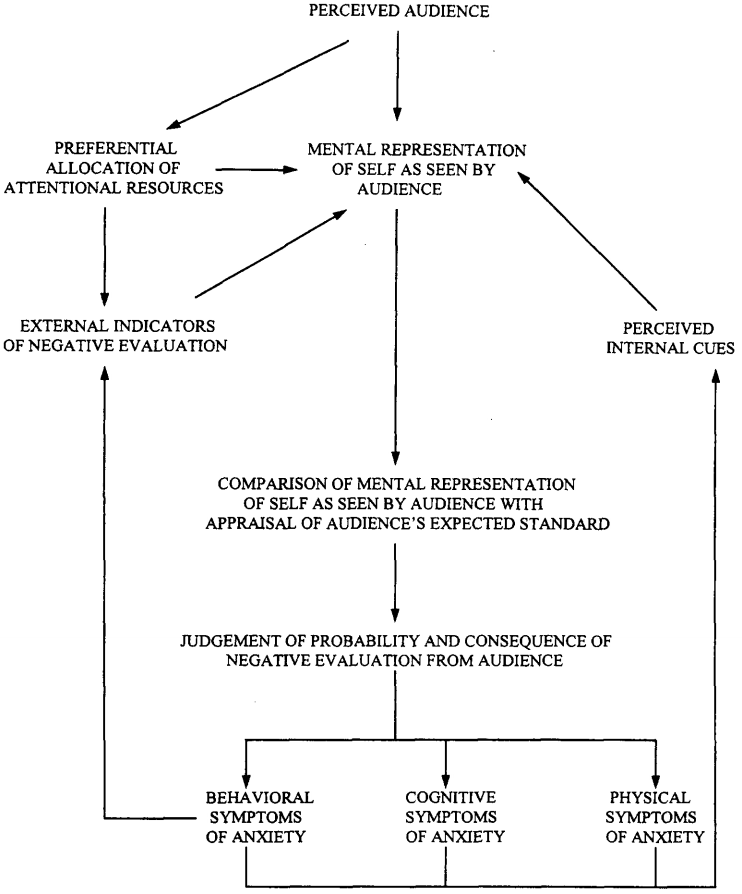
\includegraphics[scale=0.55]{Model}
	\caption{A model of the generation and maintenance of anxiety in social/evaluative situations\cite{model}.}\label{fig:model}
\end{figure}

For this reason the needs that were formulated for this are:
\begin{itemize}
	\item Have more confidence around people during the speech
	\item Listen to the speech after the performance
 external opinions.
\end{itemize}

\subsection{Constraints}
\begin{itemize}
	\item HMD;
	\item A smartphone running Android Jellybean or higher (4.1.x+);
	\item Empatica E4;
	\item Microphone;
	\item Headphones;
	\item A pc (Windows 7 or higher) with Visual C++ Redistributable Package installed
	\item Bluegiga Bluetooth Smart Dongle
	\item Comfortable place where the user can sit down and rest the arm
\end{itemize}

\subsection{Goals}
\begin{itemize}
	\item Improve the ability to speak in public
	\item Allow the subject to be less anxious before and during the speech
\end{itemize}



